
\documentclass{beamer}

\usepackage{graphicx}
\usepackage[light]{FiraSans}
\usepackage[british]{datetime2}
\usepackage{tabularx}	
\usetheme{default}
\setbeamertemplate{navigation symbols}{} % No navigation symbols
\definecolor{ntnu}{cmyk}{100,75,0,5}
\setbeamercolor{alerted text}{fg=ntnu}
\setbeamercolor{frame title}{fg=ntnu}
\setbeamercolor{title}{fg=ntnu}
\setbeamercolor{subtitle}{fg=ntnu}
\setbeamercovered{transparent}

%\setbeamertemplate{itemize item}{\color{white}$\bullet$} 
% Include above line to remove bullet indicators

\setbeamertemplate{footline}{
\begin{tabularx}{\textwidth} {
	 >{\raggedright\arraybackslash}X 
  	 >{\centering\arraybackslash}X 
  	 >{\centering\arraybackslash}X 
  	 >{\centering\arraybackslash}X 
  	 >{\centering\arraybackslash}X 
  	 >{\centering\arraybackslash}X}
	
	\raisebox{-0.3cm}
	{
\includegraphics[width=2cm, keepaspectratio]{logo_ntnu_u-slagord.pdf}} &
	\insertshortauthor & 
	\insertshorttitle &
	\insertdate &
	\insertsection &
	$\big|$ \insertframenumber
\end{tabularx}
}

\makeatletter
\makeatother

%----------------------------------------------------------------------------------------
%	TITLE PAGE
%----------------------------------------------------------------------------------------

\title[POL2012]{POL2012 Theories and models in political economy}

\subtitle{Economic inequality}

\author[Wishman]{Marius Swane Wishman} 
\date{\today} 
\institute{ISS}

\begin{document}

\begin{frame}[plain]
\titlepage 
\centering

\includegraphics[width=5cm]{logo_ntnu_u-slagord.pdf} 
\end{frame}

\section{First Section} 

\begin{frame}
\frametitle{Lessons from term papers}

\begin{itemize}
	\item[-] What is theory? \pause
	\item[-] The easiest way to deal with a carbon tax \pause
	\item[-] Less or even no protection would not necessarily spell the end
		of Norwegian agriculture (be careful with your assumptions).
\end{itemize}
	
\end{frame}
\section{Inequality}

\begin{frame}{Inequality of what?}
\begin{itemize}    
    \item[-]Gender?\pause
    \item[-]Opportunity?\pause
    \item[-]Social inequality\pause
    \item[-]Wealth?\pause
    \item[-]Income?
\end{itemize}{}
\end{frame}{}

\section{Discuss}
\begin{frame}{}
\centering
\alert{\Large{``The rich are getting richer, and the poor are getting poorer"}}
\end{frame}{}

\begin{frame}{}
\begin{itemize}
    \item[-]The economy is not a zero sum game \pause
    \item[-]``Everyone" are getting richer, but the rich are getting richer faster and some started with more\pause
    \item[-]Inequality $\neq$ Poverty
\end{itemize}{}
\end{frame}{}

\section{Empirics}

\begin{frame}{Let's look at the data} 
\begin{figure}
    \centering
    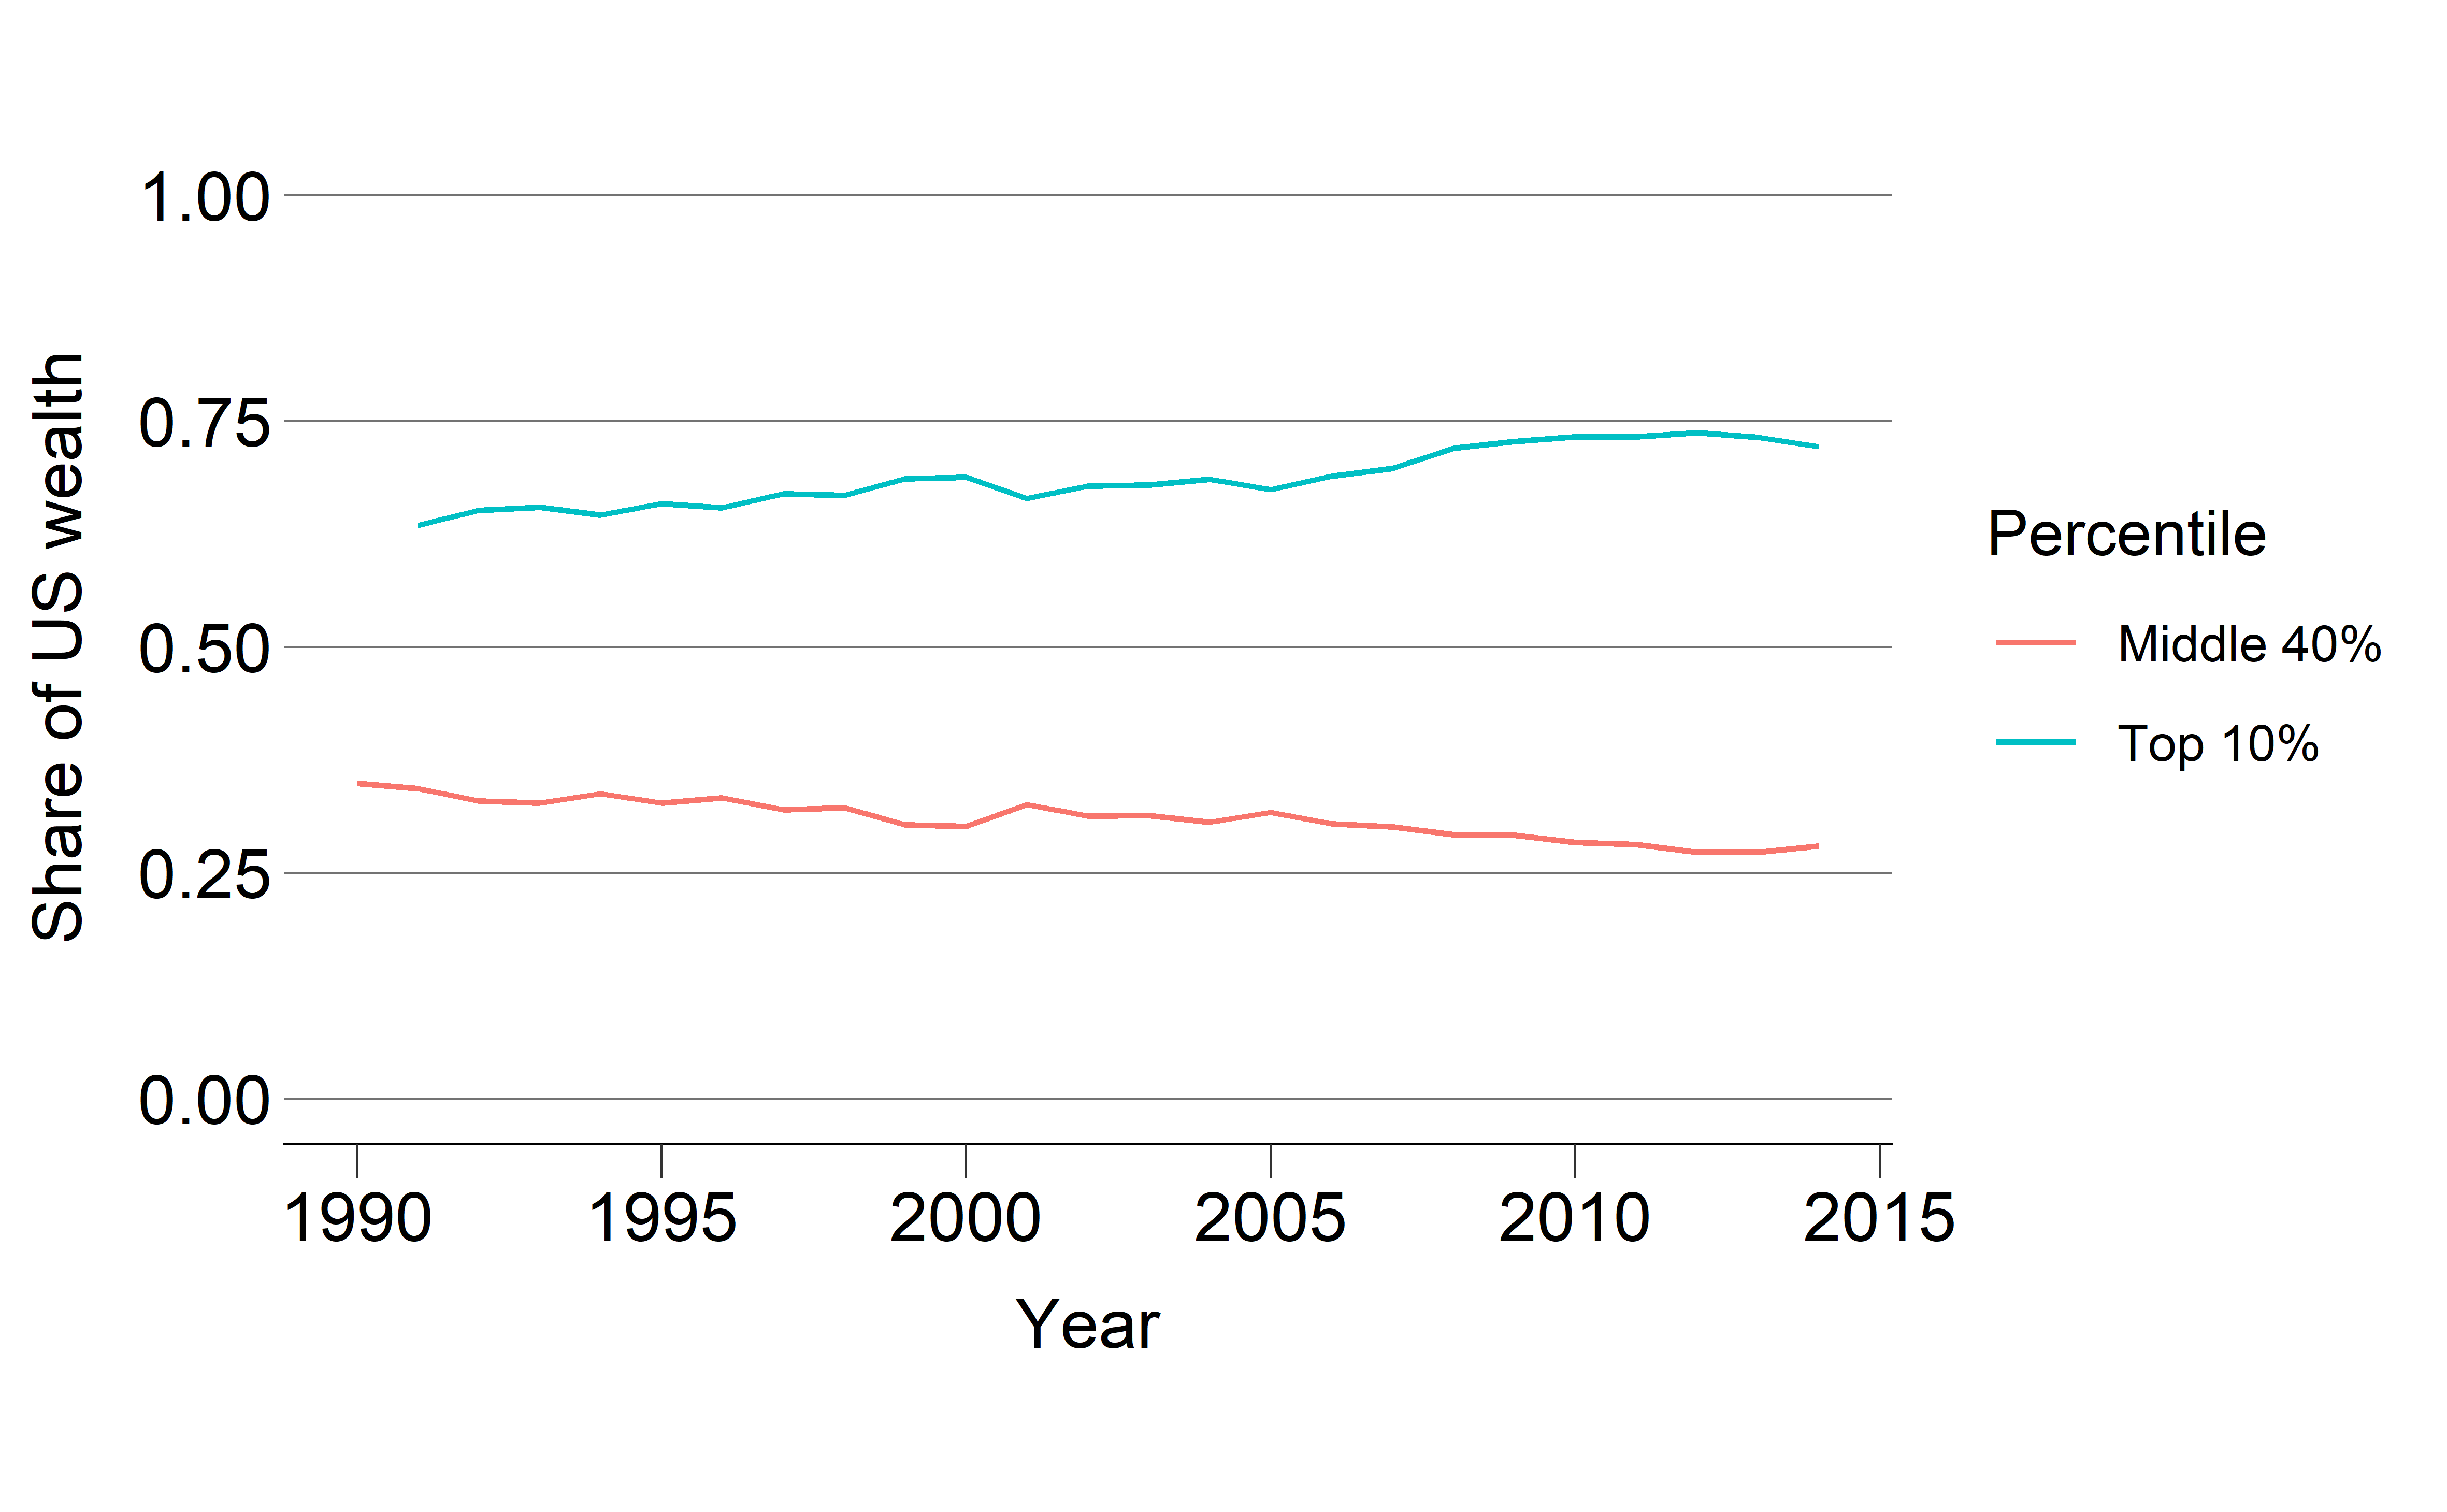
\includegraphics[width=\textwidth]{../img/InequalityUS.png}
    \caption{American Wealth inequality (Source: WID)}
\end{figure}
\end{frame}{}

\begin{frame}{Let's look at the data} 
\begin{figure}
    \centering
    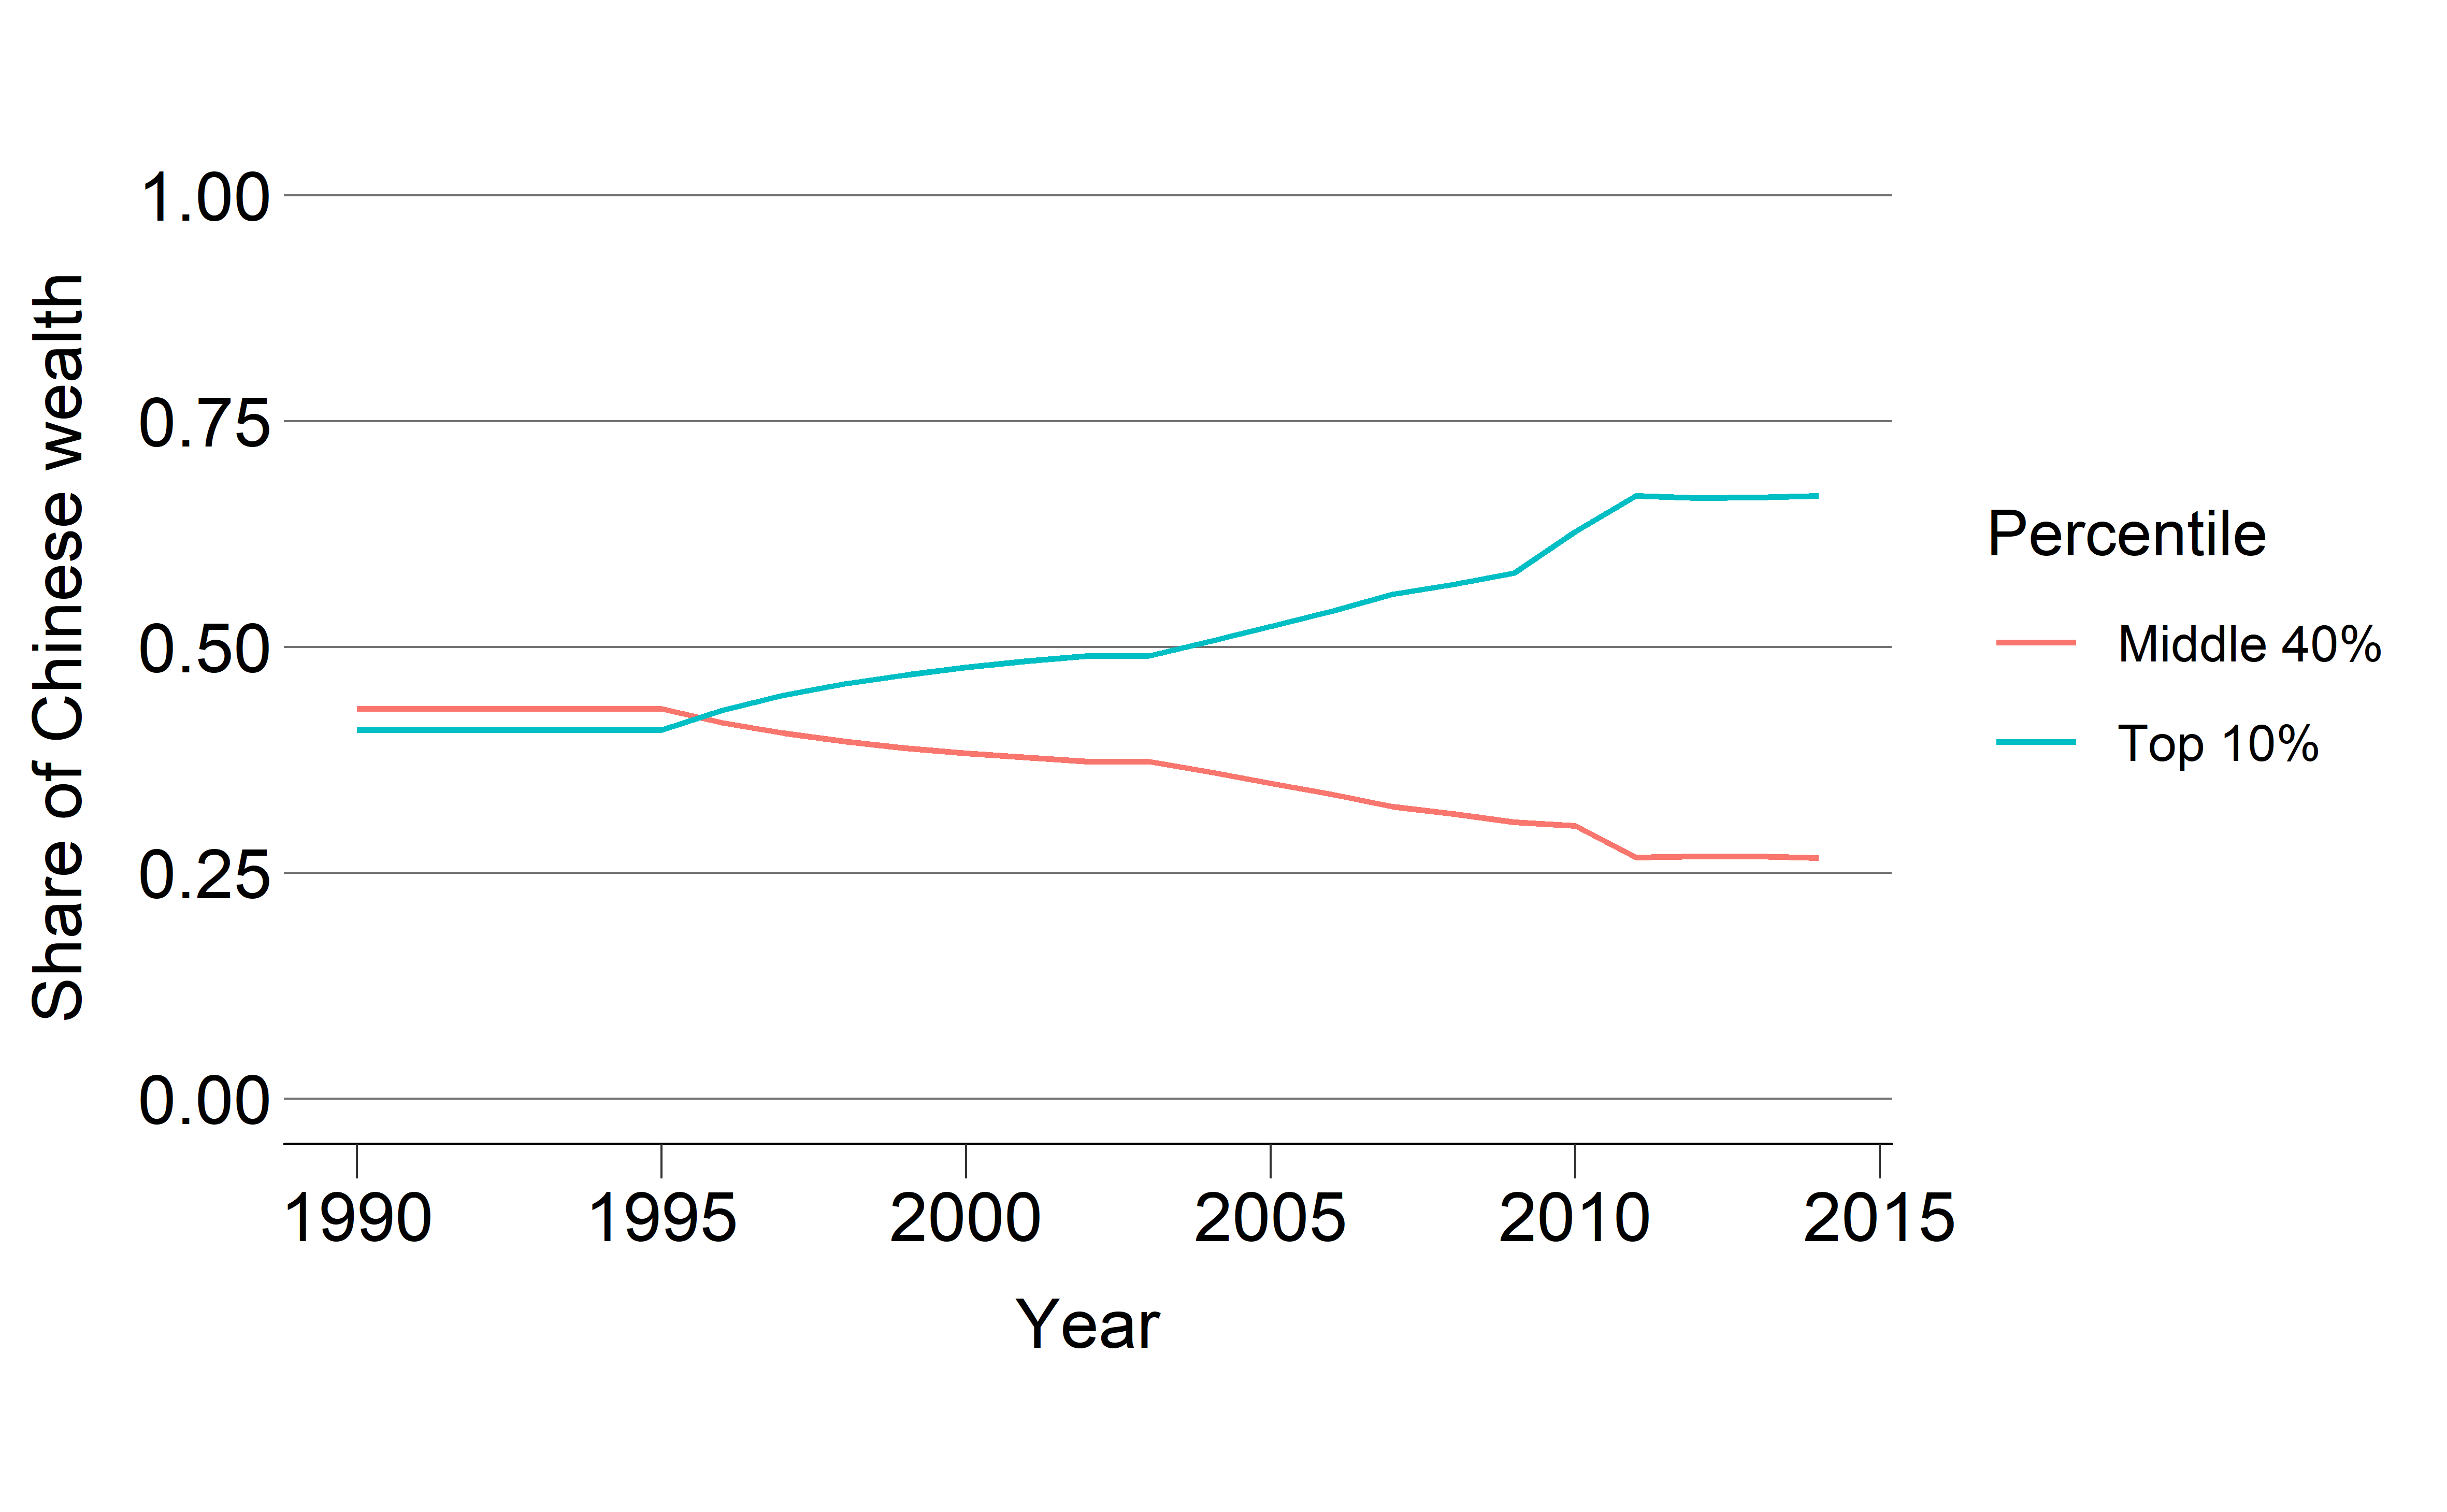
\includegraphics[width=\textwidth]{../img/InequalityCN.png}
    \caption{Chinese Wealth inequality(Source: WID)}
\end{figure}
\end{frame}{}

\begin{frame}{Top and bottom} 
\begin{figure}
    \centering
    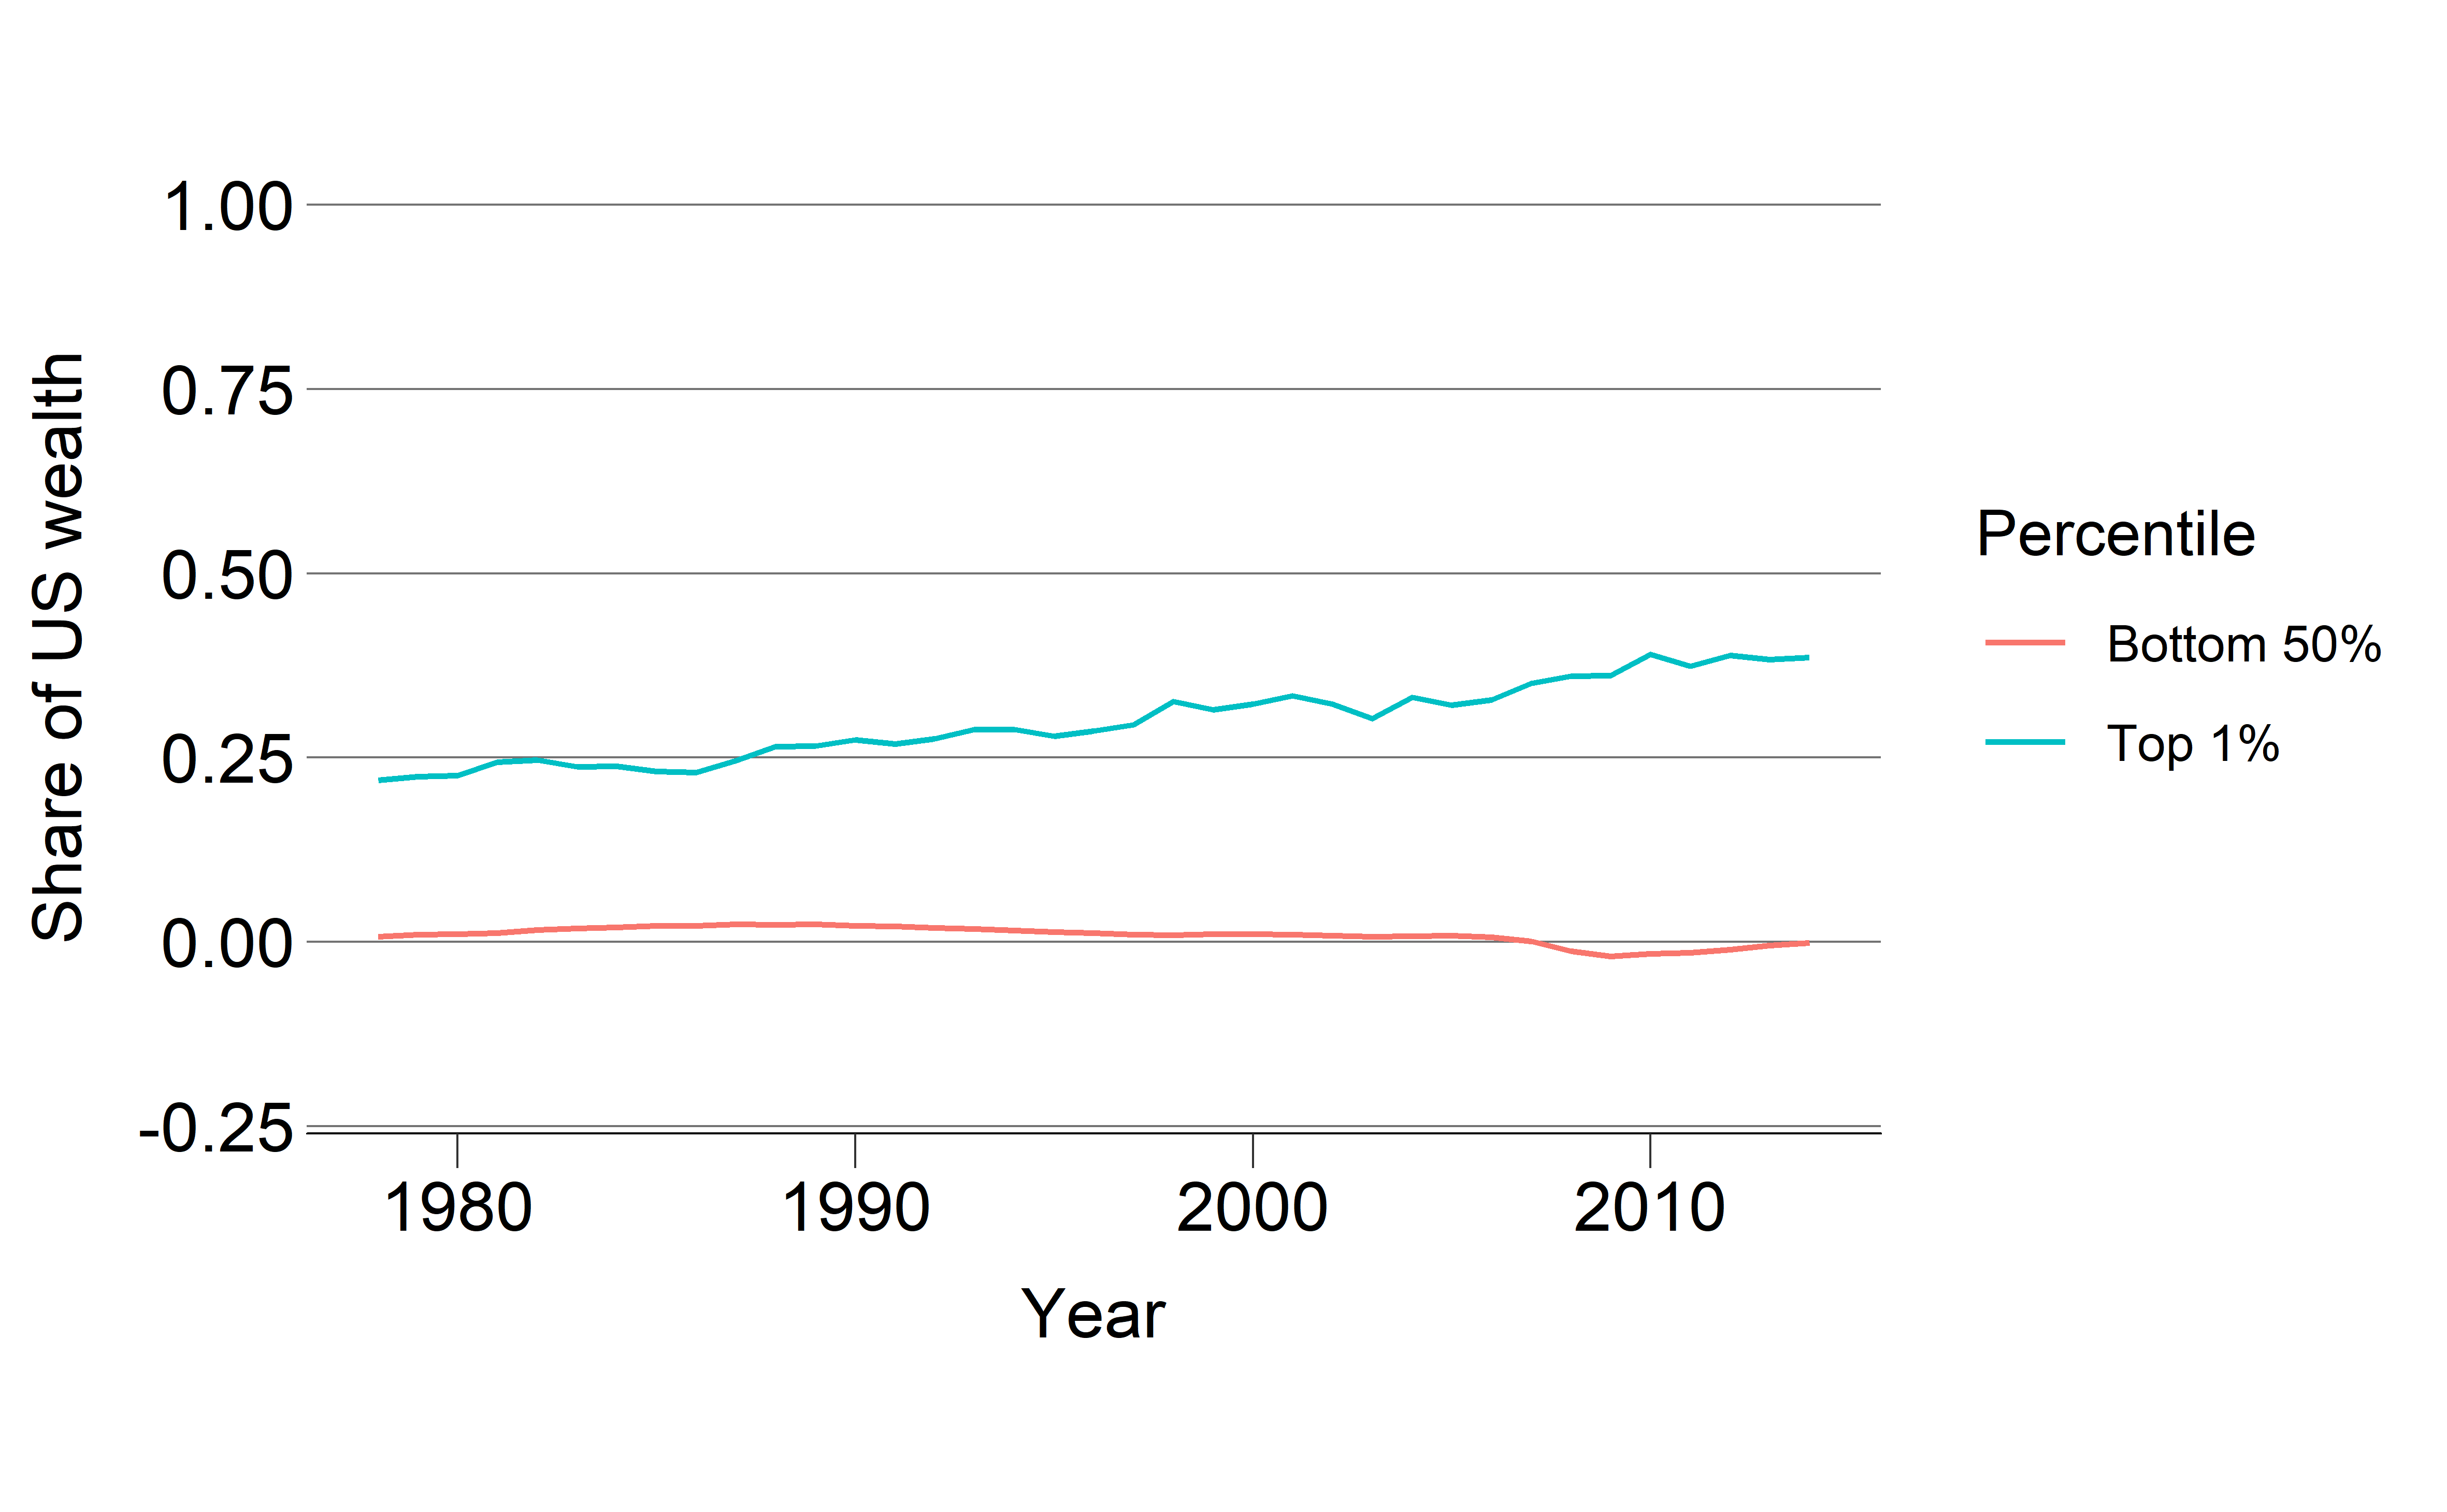
\includegraphics[width=\textwidth]{../img/InequalityTopUS.png}
    \caption{American Wealth inequality (Source: WID)}
\end{figure}
\end{frame}{}

\begin{frame}{Top and bottom} 
\begin{figure}
    \centering
    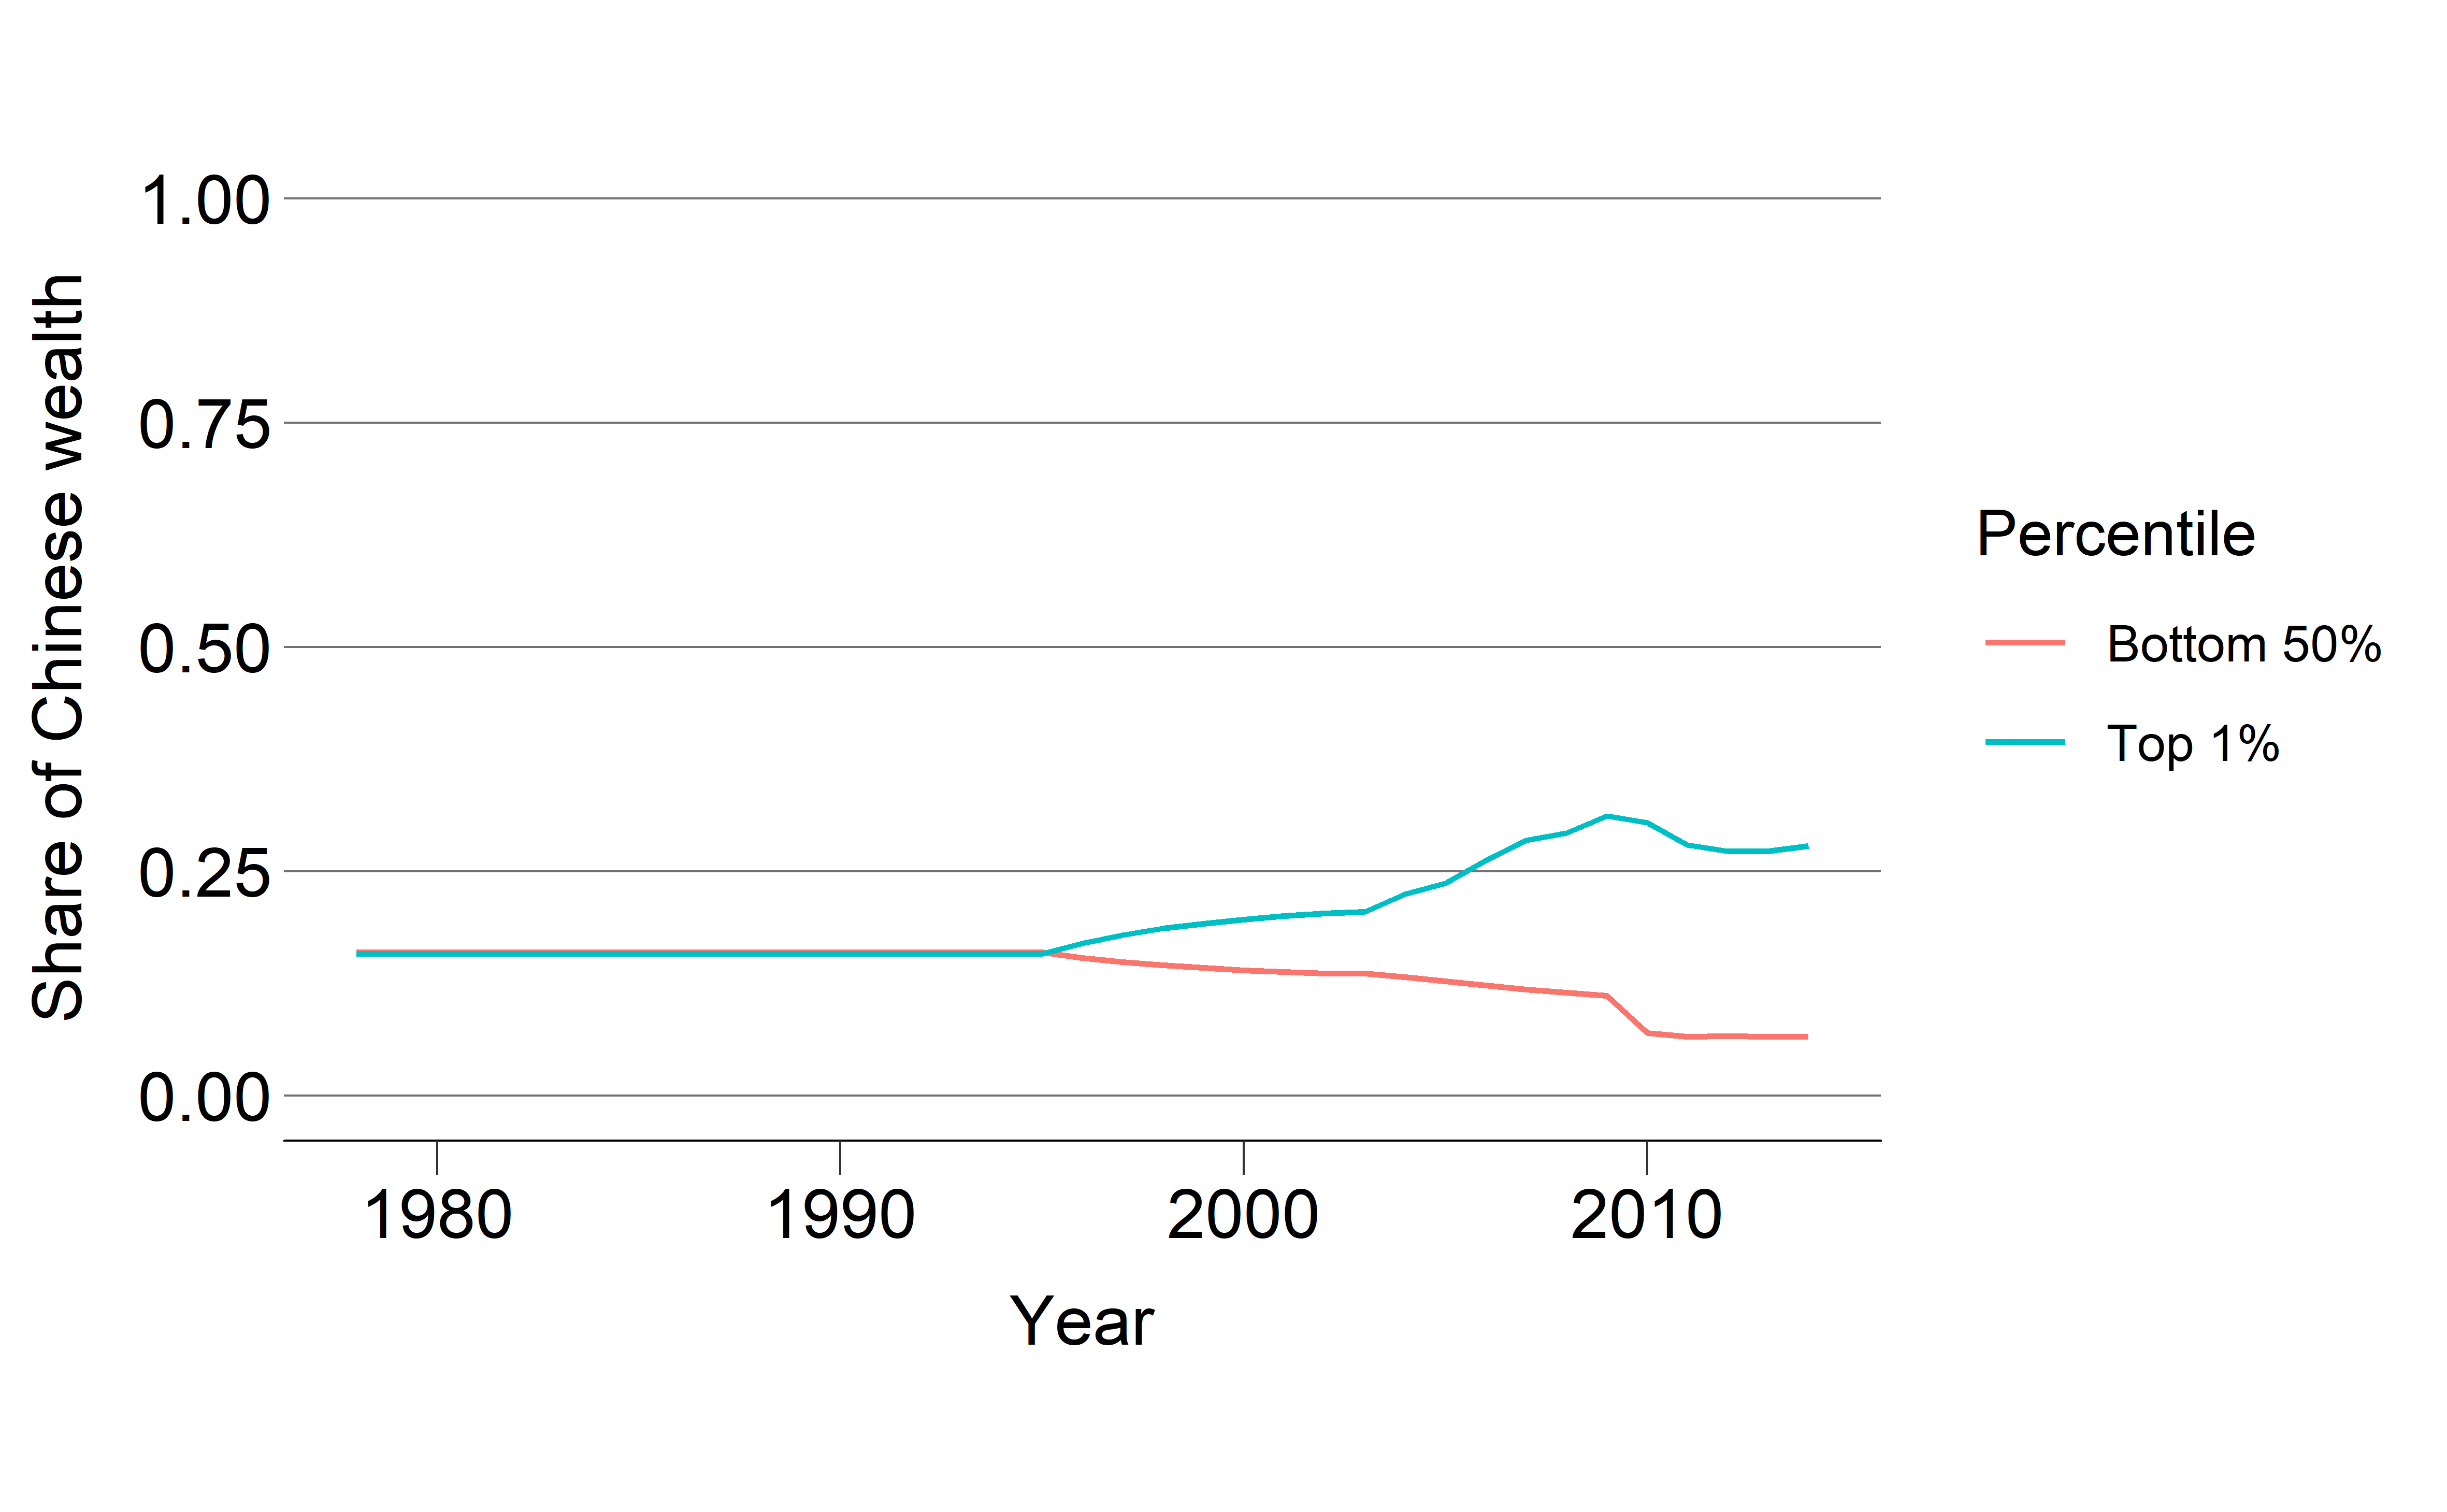
\includegraphics[width=\textwidth]{../img/InequalityTopCN.png}
    \caption{Chinese Wealth inequality (Source: WID)}
\end{figure}
\end{frame}{}

\begin{frame}{Top and bottom, Income} 
\begin{figure}
    \centering
    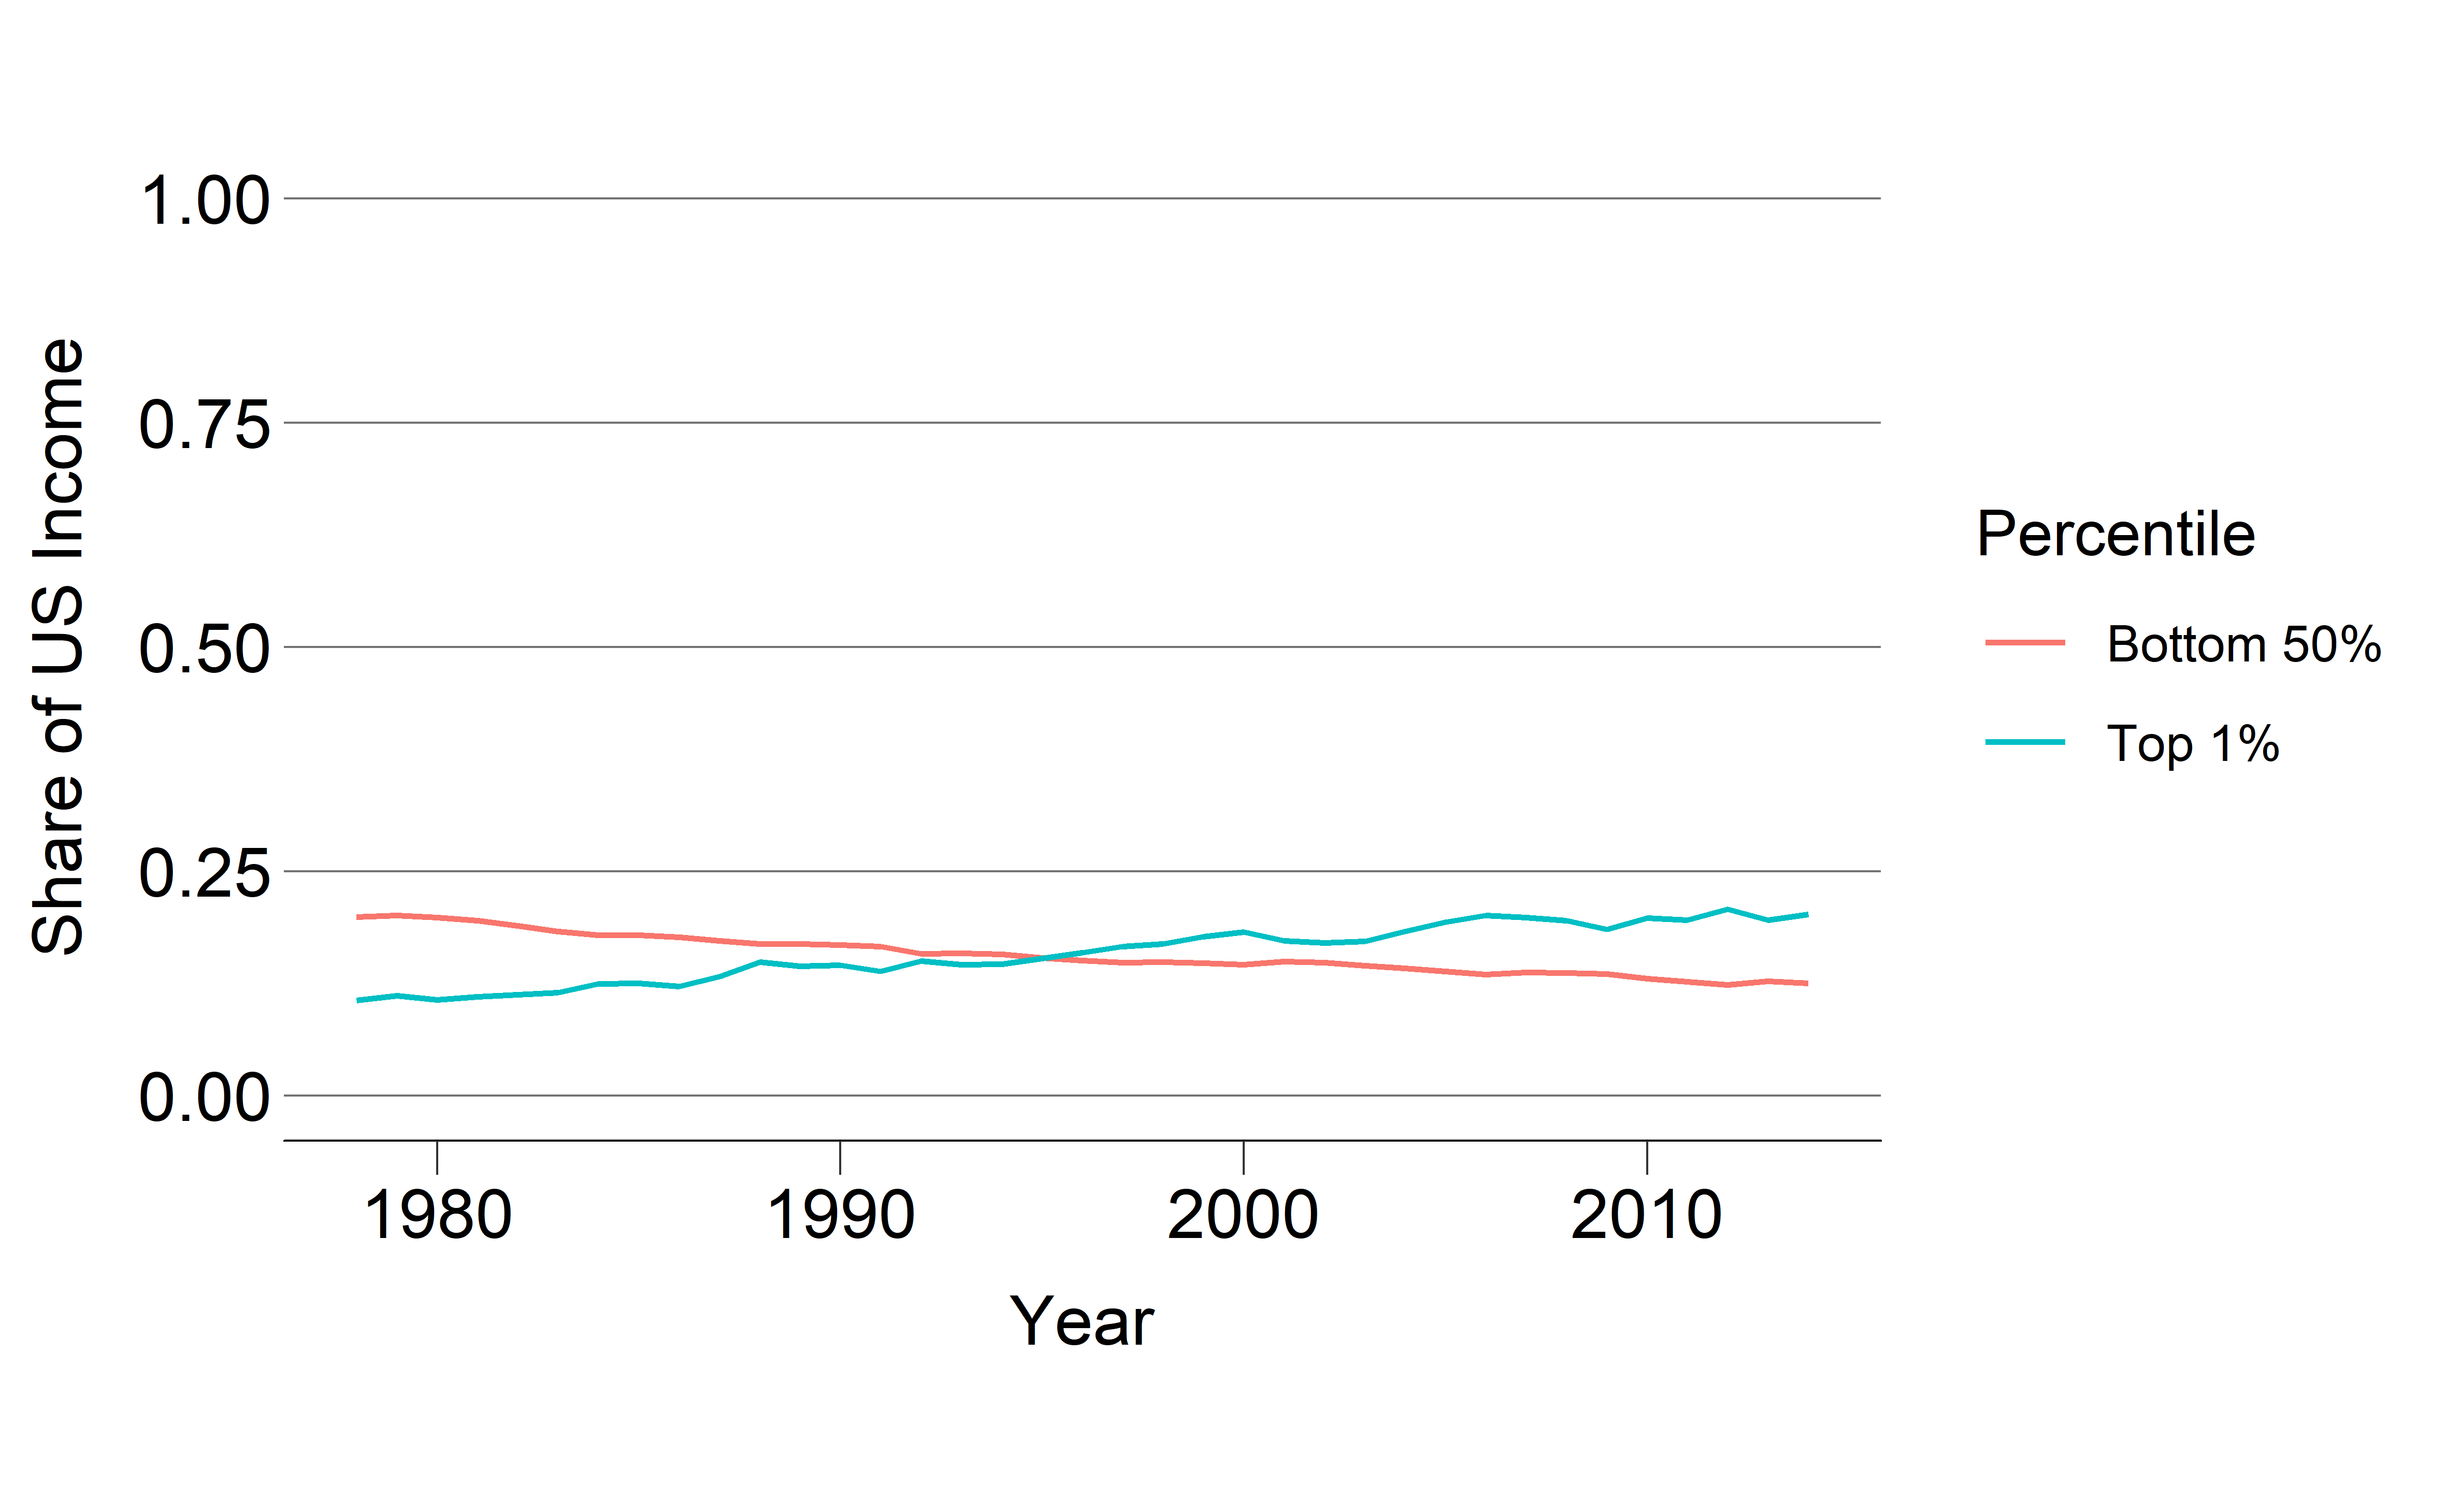
\includegraphics[width=\textwidth]{../img/InequalityIncUS.png}
    \caption{American Income inequality (Source: WID)}
\end{figure}
\end{frame}{}

\begin{frame}{Top and bottom, Income} 
\begin{figure}
    \centering
    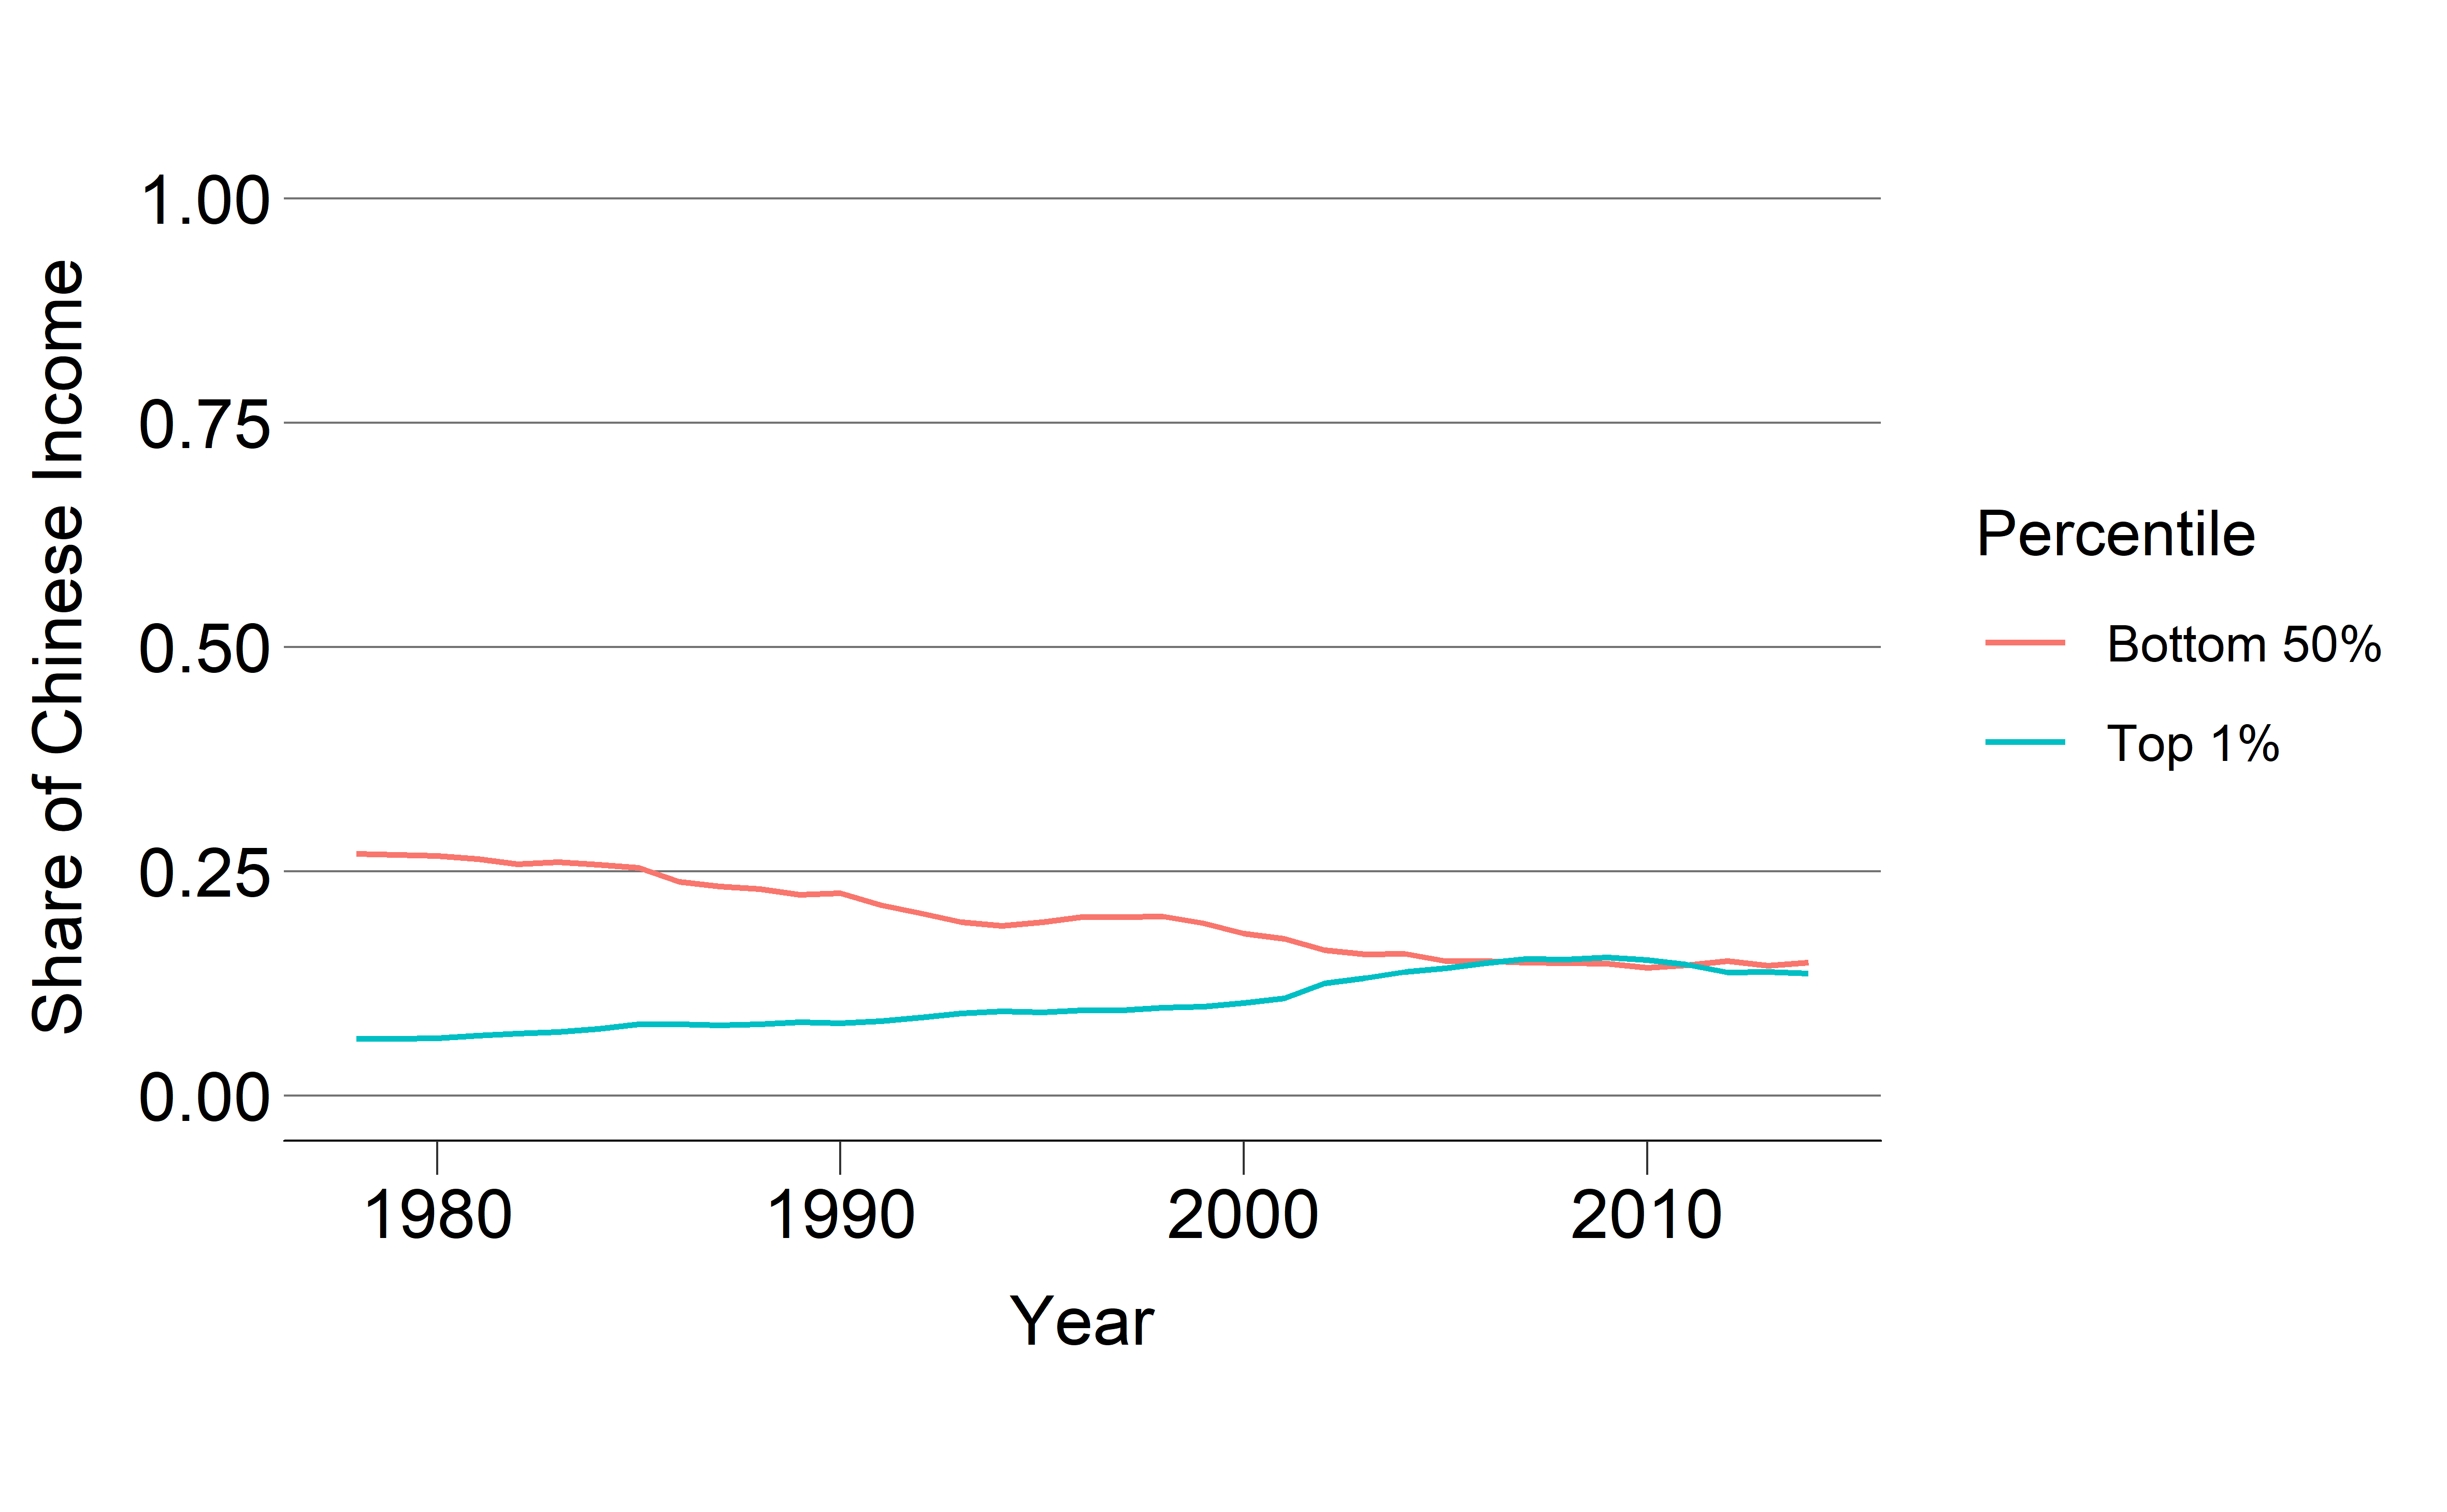
\includegraphics[width=\textwidth]{../img/InequalityIncCN.png}
    \caption{Chinese Income inequality (Source: WID)}
\end{figure}
\end{frame}{}

\begin{frame}{Poverty} 
\begin{figure}
    \centering
    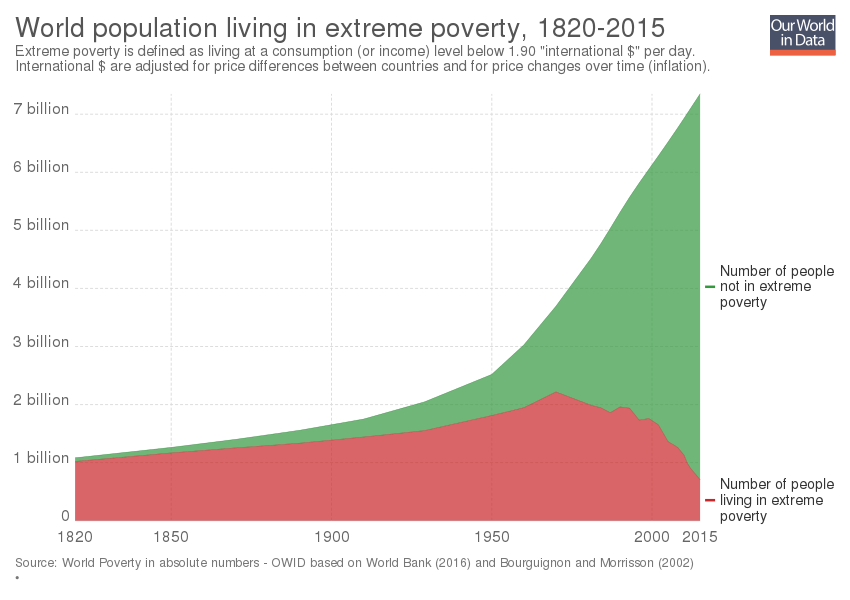
\includegraphics[width=\textwidth]{../img/poverty.png} 
    % Remember: EXTREME poverty, barely surviving, is the default human condition
\end{figure}
\end{frame}{}

\section{Theory: Consequences?}

\begin{frame}{}
\centering
\alert{\Large{What are the consequences of high/increasing economic inequality?}}

% AKA why should we care?

% No fair! Why? As long as the wealth was obtained legally, and in well
% functioning liberal democracies that is usually the case, would it not be more
% unfair to expropriate it?

% "Purely" politically problematic? Trust? 

% Remember your paradigms!
%     Marx: continued/worsening oppression of the working class (not the most
% relevant)
%     Institutionalist: money is power, power can be used to skew markets &
% politics -> growth! From meritocracy to plutocracy? (most relevant)
%     Neo-classical: reflects ability or accumulated ability, but should not
% affect equality of opportunity! -> growth, but trying to correct can also be
% problematic (relevant on consequences, but not solutions)
%     Keynes? Not (the most) relevant?
%     Evo: social upheaval/revolution, Protest parties and democratic 
% degeneration, Erodes social cohesion, reduces trust and legitimacy

% Health? Social inequality
\end{frame}{}

\section{Theory: Causes?}

\begin{frame}{}
\centering
\alert{\Large{What are the causes?}}
\end{frame}

\begin{frame}{Piketty}
\begin{columns}
\column{0.5\textwidth}
\begin{itemize}
    \item[-]$r>g$\pause
    \begin{itemize}
        \item[-]$\rightarrow$ income from rents increase more than income from wages (which depend on growth)\pause
        \item[-]$\rightarrow$ wealth inequality over time
    \end{itemize}{}
\end{itemize}{}
\column{0.5\textwidth}
\begin{figure}
    \centering
    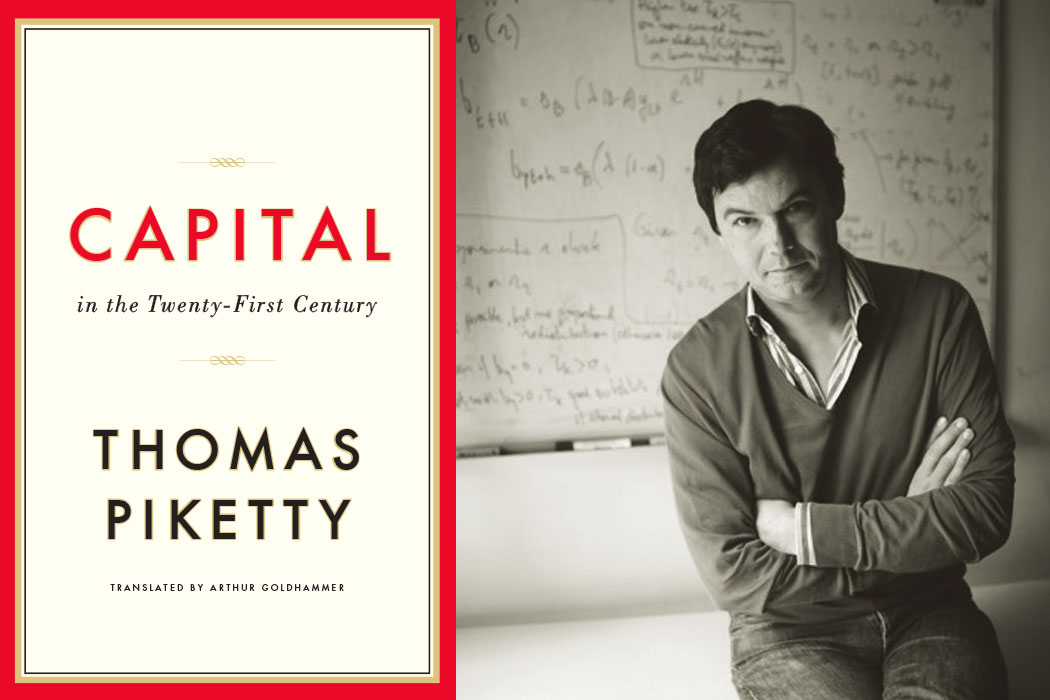
\includegraphics[width=\textwidth]{../img/PikettyCapital.jpg}
\end{figure}{}
\end{columns}
\end{frame}{}

\begin{frame}{Piketty}
\begin{columns}
\column{0.5\textwidth}
\begin{itemize}
    \item[-]$r>g$
    \item[-]Goes(2016): Observed increases in income inequality largely uncorrelated with changes in $r-g$.\pause
    \item[-]Acemoglu \& Robinson (2015): Institutions! $r>g$ not unimportant (does lead to more inequality), but many other variables quantitatively more important\pause
    \item[-]Stiglitz: Two forms of capital
\end{itemize}{}
\column{0.5\textwidth}
\begin{figure}
    \centering
    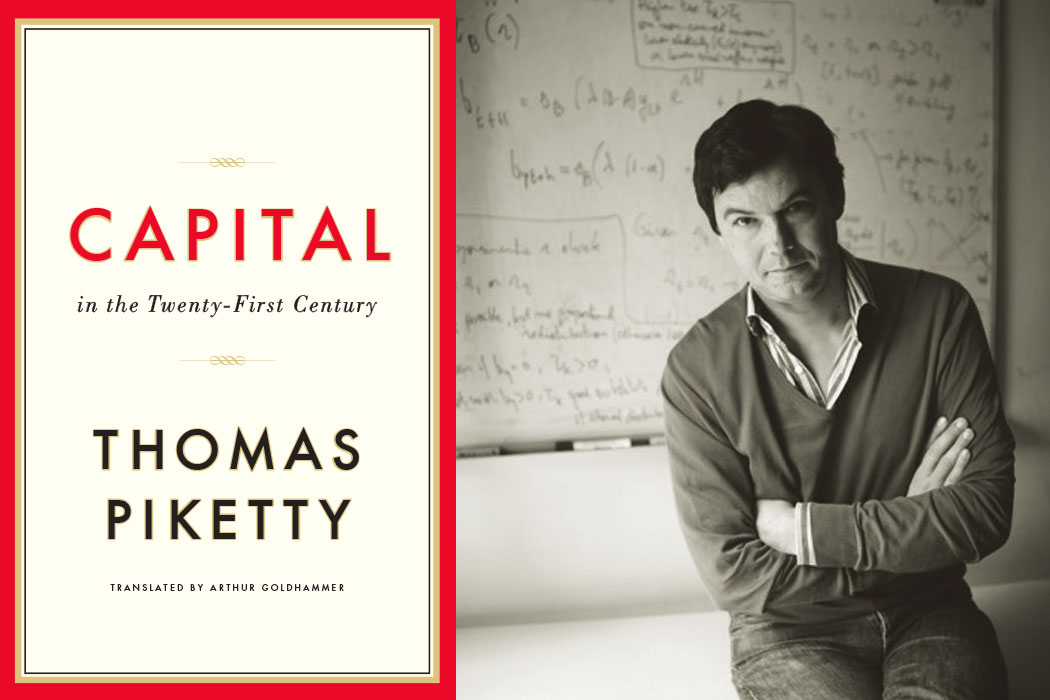
\includegraphics[width=\textwidth]{../img/PikettyCapital.jpg}
\end{figure}{}
\end{columns}
\end{frame}{}


\section{Theory: Solutions?}

\begin{frame}{}
\centering
\alert{\Large{How do we solve it?}} % Now that we care
\end{frame}

\begin{frame}{}
\begin{itemize}
    \item[-] Expropriation? \pause
    \item[-]Progressive taxation? \pause
    \begin{itemize}
        \item[-]Scheidel (2017): Only large scale violence and plague has ever worked\pause
        \item[-]Piketty: wars made the necessary policies politically viable\pause
    \end{itemize}{}
    \item[-]Public tax records?\pause
    \item[-]Global cooperation\pause
    \item[-]Focus on reducing poverty instead?
\end{itemize}{}
\end{frame}{}
\end{document}	
